\section{Grundlagen} 

\subsection*{Truncated Signed Distance Field - TSDF}

\begin{frame}[t]
    \frametitle{Grundlagen: Truncated Signed Distance Fields - TSDF}

    \begin{columns}[t]
      \column[]{7cm}
      
      \begin{itemize}
       \item Signed distance function $\Phi: \mathbf{R}^3 \to \mathbf{R}$ \\ $\rightarrow$ Distanz von Voxel zu Objektoberfläche
       \item $\Phi$ überschreitet Schwellwert $\tau$ \\ $\rightarrow$ Wird abgeschnitten 
      \end{itemize}
      \begin{equation*}
	      \Phi_{\tau}(\mathbf{x}) =
	      \begin{cases}
		      \Phi(\mathbf{x}) &  \text{wenn } | \Phi(\mathbf{x})| < \tau \\
		      \text{undefiniert} & \text{sonst}
	      \end{cases}
      \end{equation*}    
      \begin{itemize}
       \item  Gewicht vom Voxel: Gewissheit der SDF-Schätzung
       \item  Oberflächenverlauf implizit beschrieben
       \item Ermöglicht hochqualitative Oberflächen
      \end{itemize}
     

      \column{5cm}
      
    \begin{figure}[t]
      %\centering
      \vspace{-1cm}
      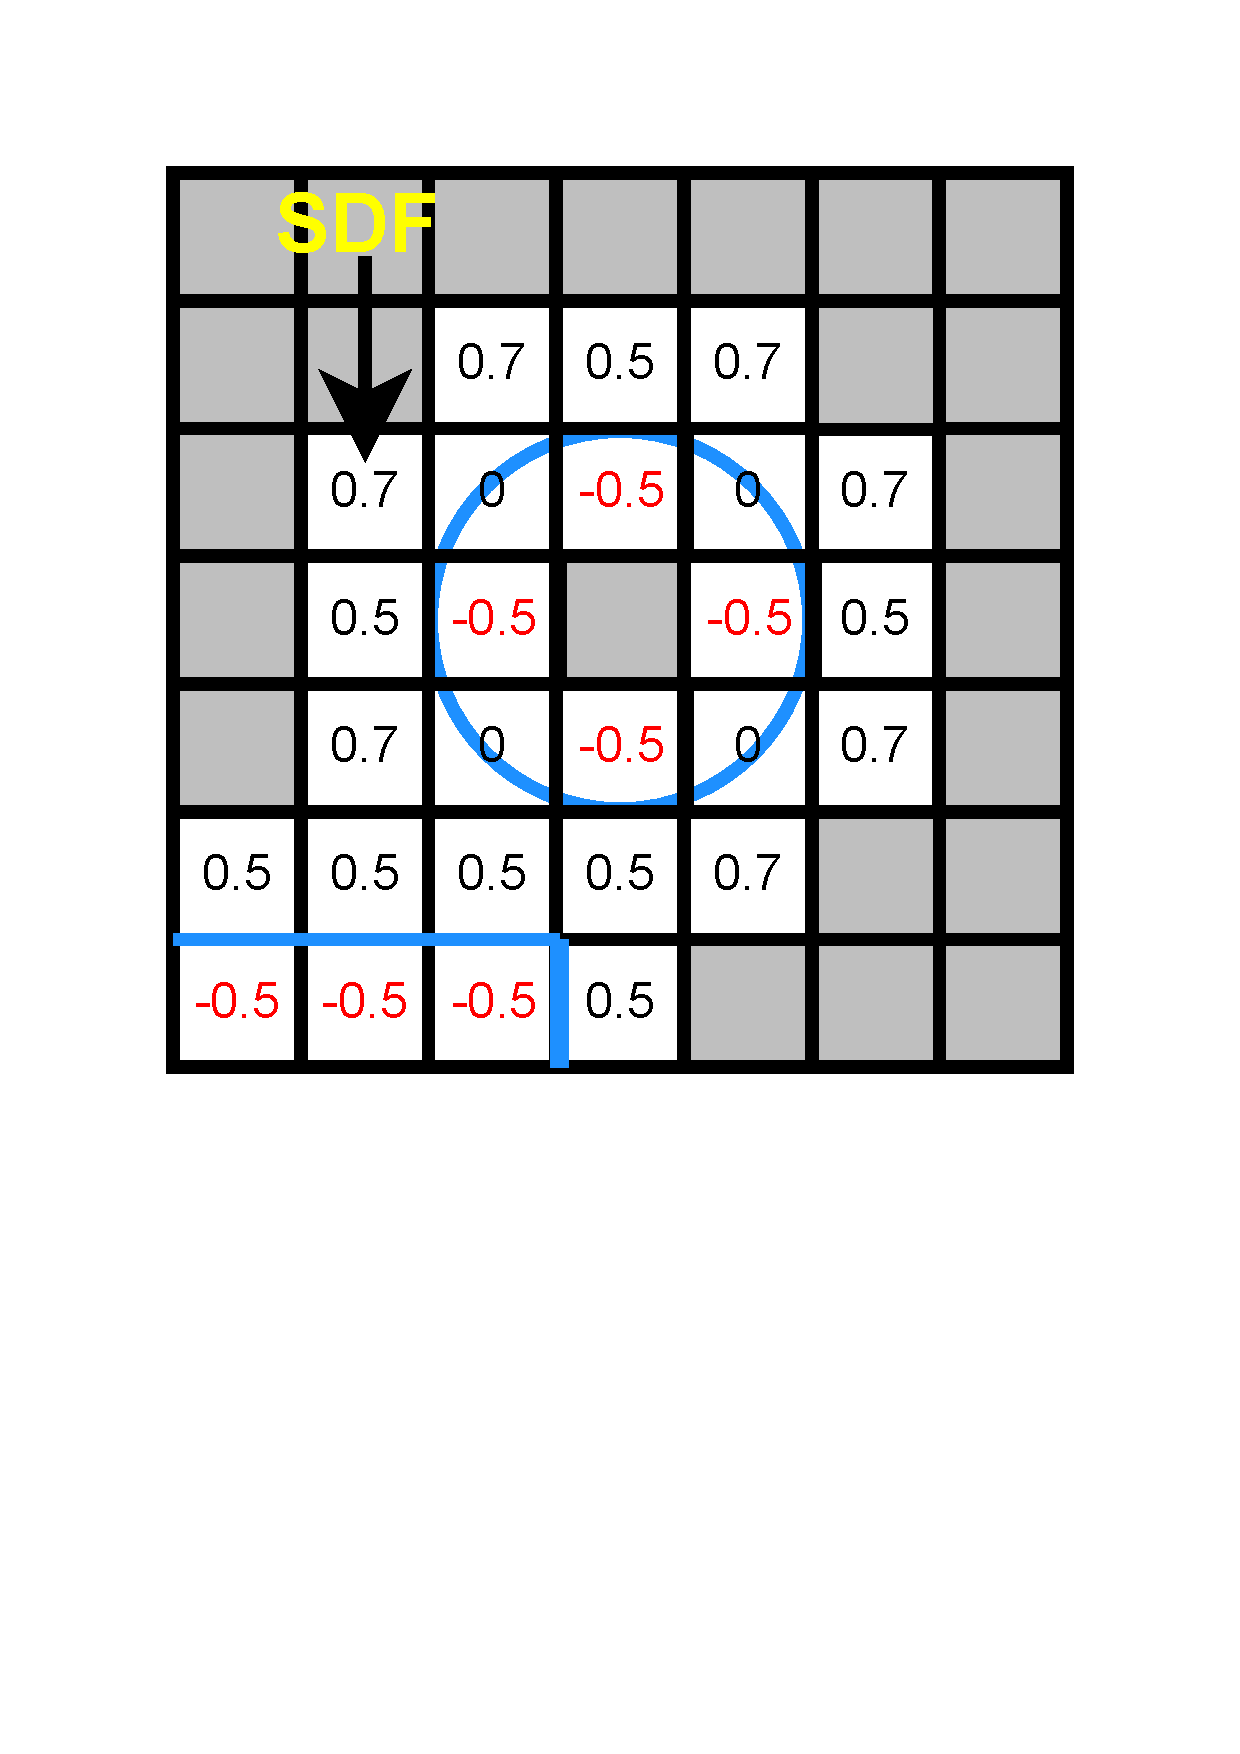
\includegraphics[trim=0 300 0 0, clip, width= \textwidth]{diagrams/tsdf.pdf}
      \caption{2D-TSDF-Voxelgitter} 

    \end{figure}
  
    \end{columns}
    \end{frame}

    \subsection*{Spatially-hashed TSDF}
    
    \begin{frame}[t]
    \frametitle{Grundlagen: Spatially-hashed TSDF}

    \begin{columns}[t]
      \column[]{7cm}
      
      \begin{itemize}
       \item TSDF in Voxelgitter: Sehr speicher- und rechenaufwändig \\ $\rightarrow$ spatially-hashed TSDF
       \item Ausnutzung dünnbesetzter Struktur
       \item Aufteilung der Szene in Voxelblöcke%, die mit Hashtabelle verwaltet  werden
       \item Nur Blöcke mit gültigen TSDF-Daten werden gespeichert
       \item Zugriff auf Voxel bei gegebener Weltposition: $\mathcal O(1)$
      \end{itemize}
     

      \column{5cm}
      
       \begin{figure}[h]
 	\centering
 	    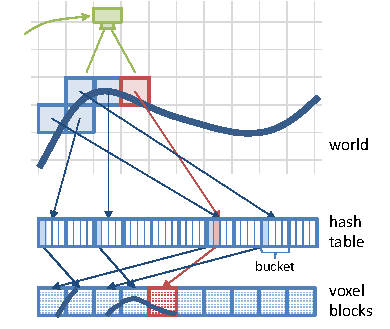
\includegraphics[width=\textwidth]{images/voxel_hashing.pdf}
 	\caption{Aufteilung der Szene in gehashte Voxelblöcke [1]} 
       \end{figure}
  
    \end{columns}
    \end{frame}